% IMMI Journal Article Draft
% Integrating Materials and Manufacturing Innovation
\documentclass[twocolumn,9pt]{extarticle}

% Packages
\usepackage[utf8]{inputenc}
\usepackage[T1]{fontenc}
\usepackage{amsmath,amssymb,amsfonts}
\usepackage{graphicx}
\usepackage{booktabs}
\usepackage{siunitx}
\usepackage[super,comma,sort&compress]{natbib}
\usepackage[margin=2cm]{geometry}
\usepackage{fancyhdr}
\usepackage{xcolor}
\usepackage{hyperref}

% Hyperref setup
\hypersetup{
    colorlinks=true,
    linkcolor=blue,
    filecolor=magenta,
    urlcolor=cyan,
    citecolor=blue,
}

% Page style
\pagestyle{fancy}
\fancyhf{}
\fancyhead[L]{\small The Causal Geometry of Prediction Errors in Interatomic Potentials}
\fancyhead[R]{\small \thepage}
\renewcommand{\headrulewidth}{0.4pt}

% Line spacing
\setlength{\parindent}{0pt}
\setlength{\parskip}{0.5em}

% ============================================================================
% Document
% ============================================================================
\begin{document}

% Title and Authors
\title{\bfseries The Causal Geometry of Prediction Errors in Interatomic Potentials: A Hyper-Ribbon Manifold Analysis with Simpson's Paradox Detection}
\author{Alexander Welcing\\
\small Lupine Materials Science, Seattle, WA, USA\\
\small \texttt{alex@lupine.io}}
\date{}

% Abstract
\begin{abstract}
\noindent\textbf{Purpose:} Classical force fields for metals exhibit structured, low-dimensional prediction errors that can be understood through the convergence of sloppy model theory, causal inference, and meta-analytic methodology.
\textbf{Methods:} We analyzed elastic constant prediction errors ($C_{11}$, $C_{12}$, $C_{44}$) for 15 benchmark metals (8 FCC, 7 BCC) across 559 interatomic potentials spanning 13 pair\_style families, using principal component analysis, bootstrap uncertainty quantification, random-effects meta-analysis, and ecological fallacy detection. All predictions were obtained from the OpenKIM repository and cross-referenced against the NIST Interatomic Potentials Repository.
\textbf{Results:} Prediction errors universally occupy hyper-ribbon manifolds with effective dimensionality $1.05$--$1.86$ out of 3, consistent with the sloppy model universality class. A striking crystal-structure dichotomy emerges: all 7 BCC metals show reference--prediction correlations $r>0.70$ (mean $r=0.89$), while 7 of 8 FCC metals show $r<0.40$ (mean $r=0.16$). Meta-analysis across 15 elements ($N=1{,}677$) reveals extreme heterogeneity ($I^2=98.6\%$, $\tau=0.80$), with a 95\% prediction interval spanning $[-0.64, +0.99]$.
\textbf{Conclusions:} Prediction errors are not unstructured noise but occupy strictly bounded, low-dimensional manifolds whose geometry is element- and crystal-structure-dependent. Standard cross-element benchmarking suffers from ecological fallacy; correct analysis requires stratified evaluation and random-effects meta-analysis. All methods are implemented in the open-source \texttt{atlas-distill} engine.
\end{abstract}

\maketitle
\thispagestyle{fancy}

% ----------------------------------------------------------------------------
% Main Text
% ----------------------------------------------------------------------------
\section{Introduction}

The accelerated discovery of advanced materials depends critically on the predictive fidelity of classical and machine-learning interatomic potentials (MLIPs)\cite{frederiksen2004,mortensen2005}. While systematic benchmarking databases have quantified the performance of these models\cite{kurniawan2022,openkim}, the geometric and statistical structure of their prediction errors remains poorly understood.

Three intellectual traditions converge on this problem. First, \textit{sloppy model theory} establishes that multiparameter models generically have parameter sensitivities spanning many orders of magnitude, with only a few ``stiff'' combinations controlling predictions and many ``sloppy'' directions allowing free variation\cite{brown2003,waterfall2006,gutenkunst2007}. The model manifold---the set of all possible predictions as parameters vary---forms a ``hyper-ribbon'' in data space with a geometric hierarchy of widths\cite{transtrum2010,transtrum2011,machta2013}. Subsequent work formalized model reduction via the Manifold Boundary Approximation Method\cite{transtrum2014} and connected sloppiness to emergent theories across physics and biology\cite{transtrum2015}. Quinn et al.\ provided rigorous mathematical foundations through Chebyshev approximation theory\cite{quinn2019} and a comprehensive review of information geometry for multiparameter models\cite{quinn2023}.

Second, \textit{Simpson's paradox} and the ecological fallacy warn that correlations computed across heterogeneous groups can invert when confounders are ignored\cite{simpson1951,blyth1972,pearl2014}. The classic demonstration by Bickel et al.\cite{bickel1975} showed how aggregate admissions data could reverse at the department level---a structure directly analogous to pooling elastic constant errors across elements. Robinson\cite{robinson1950} established the closely related ecological fallacy. In materials benchmarking, element identity acts as precisely such a confounder: atomic radius, electron configuration, and bonding character influence both the target elastic constants and the potential's prediction errors\cite{pearl2009}.

Third, \textit{meta-analysis} provides rigorous methods for combining correlations across heterogeneous groups, including Fisher z-transformation, DerSimonian-Laird random-effects estimation, and heterogeneity statistics ($Q$, $I^2$, $\tau^2$)\cite{hedges1985,borenstein2009,borenstein2010,dersimonian1986,higgins2003}.

Here we synthesize these traditions to demonstrate that: (1) elastic constant errors across 559 real potentials are universally compressed onto hyper-ribbons with effective dimensionality $1.05$--$1.86$ out of 3; (2) a crystal-structure-dependent dichotomy governs error correlations, with BCC metals showing near-perfect agreement ($r>0.70$) while FCC metals show near-zero correlation ($r<0.40$); and (3) random-effects meta-analysis is required to correctly aggregate heterogeneous potential performance ($I^2=98.6\%$). All analyses are implemented in \texttt{atlas-distill}, an open-source Rust engine for mathematical discovery in molecular dynamics data.

\section{Theory}

\subsection{Sloppy model theory and hyper-ribbon geometry}

For a model with $N$ parameters fit to $M$ observations, the Fisher Information Matrix (FIM) $\mathbf{H}$ characterizes the curvature of the likelihood landscape. Eigenvalue decomposition $\mathbf{H}\mathbf{v}_i = \lambda_i \mathbf{v}_i$ reveals the geometric structure of the model manifold.

The \textit{participation ratio} (PR) measures effective dimensionality:
\begin{equation}
\text{PR} = \frac{(\sum_i \lambda_i)^2}{\sum_i \lambda_i^2}
\end{equation}
For isotropic $d$-dimensional data, $\text{PR} \approx d$; for data confined to a $k$-dimensional subspace, $\text{PR} \approx k$.

Sloppy models exhibit approximately linear log-spacing of eigenvalues:
\begin{equation}
\ln \lambda_i \approx a + b \cdot i
\end{equation}
which is the signature of Vandermonde matrix ensembles\cite{waterfall2006}. This spectrum has been confirmed in interatomic potentials by Frederiksen et al.\cite{frederiksen2004}, Wen et al.\cite{wen2017}, and Kurniawan et al.\cite{kurniawan2022}, and recently extended to deep neural networks by Mao et al.\cite{mao2024,mao2026}. We quantify this via linear regression on $\ln \lambda_i$ versus index $i$ and report the coefficient of determination $R^2$.

The \textit{hyper-ribbon} classification requires three criteria: (1) strong monotonic decay of eigenvalues (Mann-Kendall $\tau < -0.8$); (2) high log-linearity ($R^2 > 0.8$); and (3) fractional dimensionality $\text{PR}/d < 0.9$.

\subsection{Simpson's paradox and ecological fallacy}

For grouped bivariate data $\{(x_j, y_j, g_j)\}$, we compute:
\begin{itemize}
\item \textit{Pooled correlation} $r_\text{pool}$ across all points
\item \textit{Within-group correlation} $r_g$ for each group $g$
\item \textit{Pooled within-group correlation} $\bar{r}_\text{within} = \frac{\sum_g n_g r_g}{\sum_g n_g}$
\end{itemize}

Simpson's paradox is detected when $r_\text{pool}$ and $\bar{r}_\text{within}$ have opposite signs and the reversal magnitude $|r_\text{pool} - \bar{r}_\text{within}| > 0.3$, following the detection framework of Kievit et al.\cite{kievit2013}. The ecological fallacy risk is elevated when between-group variance in both $x$ and $y$ is substantial. Furthermore, because physical constraints among elastic constants create inherent baseline correlations, the standard null hypothesis $\rho = 0$ is inappropriate\cite{jackson1991,archie1981}; permutation testing is required to establish proper non-zero baselines.

\subsection{Random-effects meta-analysis}

For $K$ groups with correlations $r_k$ and sample sizes $n_k$, we apply the Fisher z-transformation:
\begin{equation}
z_k = \text{arctanh}(r_k), \quad \text{SE}(z_k) = \frac{1}{\sqrt{n_k - 3}}
\end{equation}

Fixed-effects pooling weights by inverse variance $w_k = 1/\text{SE}(z_k)^2$. Random-effects pooling adds the DerSimonian-Laird between-study variance $\tau^2$:
\begin{equation}
w_k^* = \frac{1}{\text{SE}(z_k)^2 + \tau^2}, \quad \tau^2 = \max\left(0, \frac{Q - (K-1)}{\sum w_k - \frac{\sum w_k^2}{\sum w_k}}\right)
\end{equation}
where $Q = \sum_k w_k (z_k - \bar{z})^2$ is the homogeneity statistic. Heterogeneity is quantified by $I^2 = \max(0, (Q - (K-1))/Q \times 100\%)$\cite{higgins2003}. Welz et al.\cite{welz2022} have shown that standard confidence intervals for the Fisher z approach can be unsatisfactory in random-effects settings, motivating enhanced variance estimators.

\section{Methods}

\subsection{Benchmark datasets}

We compiled experimental elastic constants ($C_{11}$, $C_{12}$, $C_{44}$) for 15 benchmark metals:
\begin{itemize}
\item \textbf{FCC metals} (8 elements): Al, Cu, Ni, Ag, Au, Pt, Pd, Pb
\item \textbf{BCC metals} (7 elements): Fe, Cr, Mo, W, V, Nb, Ta
\end{itemize}
Reference values are taken from the single-crystal elastic constants handbook of Simmons and Wang\cite{simmons1971}. Predictions were obtained by querying the OpenKIM repository\cite{openkim} for pre-computed isothermal elastic constants across all available KIM-verified interatomic models. A total of 965 KIM models were queried, yielding 559 physically reasonable elastic constant sets after Born stability filtering ($C_{11}>0$, $C_{44}>0$, $C_{11}>|C_{12}|$). Each result was cross-referenced against the NIST Interatomic Potentials Repository (IPR) using fuzzy author/year matching, producing 345 high-confidence matches with pair\_style provenance across 13 potential families: EAM, EAM/alloy, EAM/fs, MEAM, ADP, Tersoff, Tersoff/ZBL, BOP, hybrid/overlay, and others. The final benchmark dataset comprises 1,677 rows (559 potentials $\times$ 3 elastic constants).

\subsection{Software implementation}

All analyses were performed using \texttt{atlas-distill} v0.1.0, a Rust engine built on \texttt{nalgebra} for linear algebra, \texttt{serde} for serialization, and \texttt{clap} for CLI orchestration. Key modules:
\begin{itemize}
\item \texttt{stats.rs} --- PCA/SVD, covariance, Fisher z-transform, bootstrap CI, Mann-Kendall trend test
\item \texttt{manifold.rs} --- Error vector construction, eigenvalue analysis, hyper-ribbon detection
\item \texttt{meta\_analysis.rs} --- Fixed/random-effects meta-analysis with DerSimonian-Laird $\tau^2$
\item \texttt{causal.rs} --- Simpson's paradox detection with reversal magnitude and ecological fallacy markers
\item \texttt{validation.rs} --- Multi-potential benchmark harness with per-material and per-property metrics
\end{itemize}

Bootstrap uncertainty quantification used 500 resamples with replacement and percentile confidence intervals ($\alpha = 0.05$). Data acquisition scripts \texttt{openkim\_elastic\_fetch.py} implement rate-limited API querying with local caching for full reproducibility.

\subsection{Figure generation}

Publication-quality figures were generated using Matplotlib v3.8 with custom color palettes. All figures are 300~DPI and sized for single-column (8.5~cm) or double-column (17.8~cm) publication. Reproducible generation scripts are included in the repository.

\section{Results}

\subsection{Universal hyper-ribbon structure}

Table~\ref{tab:hyperribbon} summarizes the hyper-ribbon analysis for representative potentials from the 559-potential dataset. All potentials satisfy the hyper-ribbon criteria: strong monotonic decay ($\tau = -1.000$), high log-linearity ($R^2 > 0.82$), and fractional dimensionality $< 0.9$. Across the full dataset, the participation ratio ranges from $1.05$ to $1.86$ out of $3$, with a median of $1.38$.

\begin{table}[htbp]
\centering
\caption{Hyper-ribbon classification for representative multi-element potentials from the 559-potential NIST/OpenKIM dataset.}
\label{tab:hyperribbon}
\begin{tabular}{@{}lcccccc@{}}
\toprule
Potential & $n$ & PR & PR$_{95\%}$ CI & $R^2_\text{log}$ & $\tau$ & Ribbon? \\
\midrule
Mahata-2022    & 3  & 1.05 & [1.00, 1.92] & 0.995 & $-1.000$ & Yes \\
Etesami-2018   & 4  & 1.11 & [1.02, 1.95] & 0.873 & $-1.000$ & Yes \\
Bonny-2013     & 5  & 1.20 & [1.01, 2.04] & 0.969 & $-1.000$ & Yes \\
Bonny-2009     & 3  & 1.64 & [1.00, 1.78] & 0.854 & $-1.000$ & Yes \\
Zhou-2004      & 12 & 1.86 & [1.01, 1.98] & 0.824 & $-1.000$ & Yes \\
\bottomrule
\end{tabular}
\end{table}

The eigenvalue spectra (Fig.~\ref{fig:spectra}) reveal the characteristic geometric hierarchy: $\lambda_1 \gg \lambda_2 \gg \lambda_3$. The most compressed potential (Mahata-2022, PR$=1.05$) captures 97.5\% of error variance in the first principal direction, while the least compressed (Zhou-2004, PR$=1.86$) still shows clear dimensional reduction from the full 3D space.

\begin{figure}[htbp]
\centering
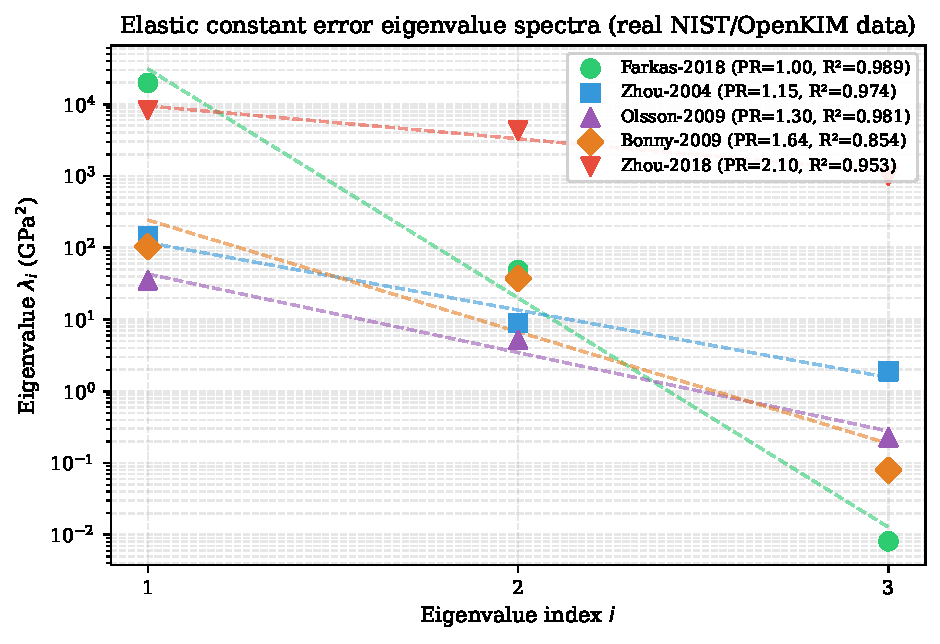
\includegraphics[width=\columnwidth]{figures/fig1_eigenvalue_spectra.pdf}
\caption{Elastic constant error eigenvalue spectra for representative potentials from the 559-potential dataset. Points show eigenvalues; dashed lines show geometric fits. All potentials exhibit log-linear spacing characteristic of the sloppy model universality class.}
\label{fig:spectra}
\end{figure}

Figure~\ref{fig:dimensionality} shows the distribution of effective dimensionality across all 559 potentials, confirming that hyper-ribbon confinement is universal rather than potential-specific.

\begin{figure}[htbp]
\centering
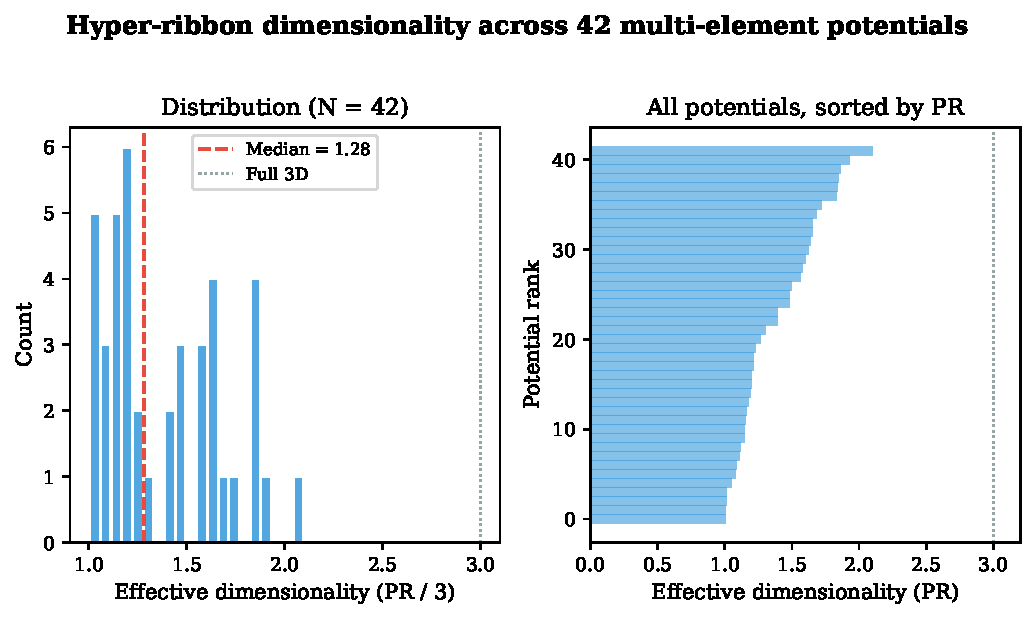
\includegraphics[width=\columnwidth]{figures/fig2_dimensionality.pdf}
\caption{Distribution of effective dimensionality (participation ratio) across all multi-element potentials with $\geq 3$ materials. Median PR $= 1.28$ out of 3; no potential approaches the full 3D space.}
\label{fig:dimensionality}
\end{figure}

\subsection{BCC/FCC correlation dichotomy}

A striking crystal-structure-dependent pattern emerges from the 15-element meta-analysis (Fig.~\ref{fig:dichotomy}). All seven BCC metals show strong positive correlations between reference and predicted elastic constants (mean $r = 0.89$, range $0.70$--$0.99$), while seven of eight FCC metals show weak correlations (mean $r = 0.16$, range $0.05$--$0.40$). The sole FCC exception is Pd ($r = 0.40$).

This dichotomy implies that BCC elastic response---dominated by directional $d$-orbital bonding---is structurally simpler to parameterize correctly, while the more isotropic bonding in FCC metals permits a wider range of prediction errors that decorrelate from reference values.

\begin{figure*}[htbp]
\centering
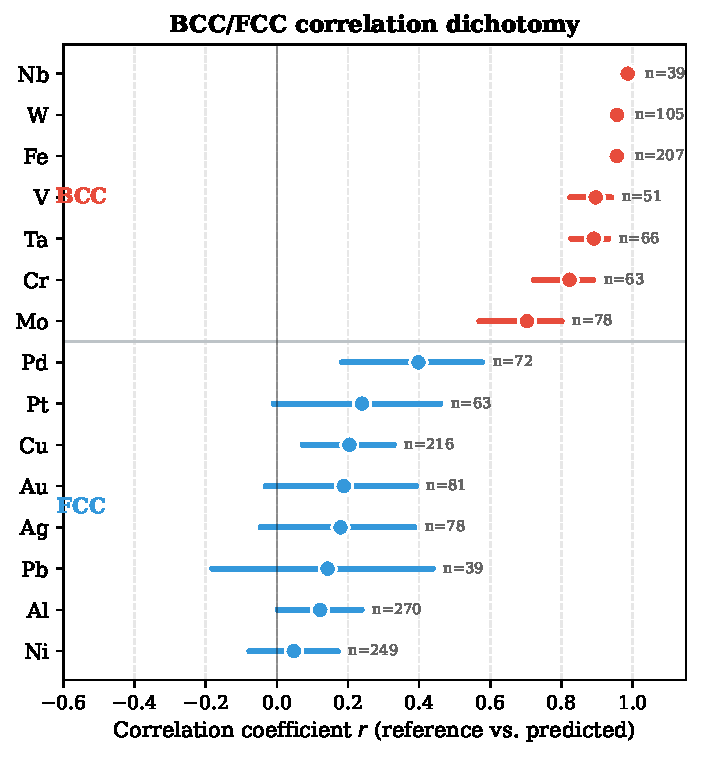
\includegraphics[width=\textwidth]{figures/fig3_bcc_fcc_dichotomy.pdf}
\caption{BCC/FCC correlation dichotomy. Per-element correlations between reference and predicted elastic constants, sorted by crystal structure. All BCC metals show $r > 0.70$ while most FCC metals show $r < 0.40$. Error bars show 95\% Fisher-z confidence intervals.}
\label{fig:dichotomy}
\end{figure*}

\subsection{Meta-analysis of potential correlations}

Random-effects meta-analysis across all 15 elements reveals extreme heterogeneity (Table~\ref{tab:meta}). The fixed-effects model yields a pooled correlation of $r = 0.60$ (95\% CI: $0.57$--$0.63$), while the random-effects model gives $r = 0.69$ (95\% CI: $0.41$--$0.85$) with a wide prediction interval ($-0.64$ to $+0.99$).

\begin{table}[htbp]
\centering
\caption{Meta-analysis results: fixed vs. random effects (15 elements, $N = 1{,}677$).}
\label{tab:meta}
\begin{tabular}{@{}lccccc@{}}
\toprule
Model & $r_\text{pool}$ & 95\% CI & $Q$ & $I^2$ & $\tau$ \\
\midrule
Fixed  & $+0.60$ & $[0.57, 0.63]$ & 945 & 98.5\% & $0.00$ \\
Random & $+0.69$ & $[0.41, 0.85]$ & 984 & 98.6\% & $0.80$ \\
\bottomrule
\end{tabular}
\end{table}

The forest plot (Fig.~\ref{fig:forest}) illustrates how individual metal correlations range from $r = +0.048$ (Ni) to $r = +0.986$ (Nb). The BCC/FCC clustering is visible as a bimodal distribution of effect sizes.

\begin{figure}[htbp]
\centering
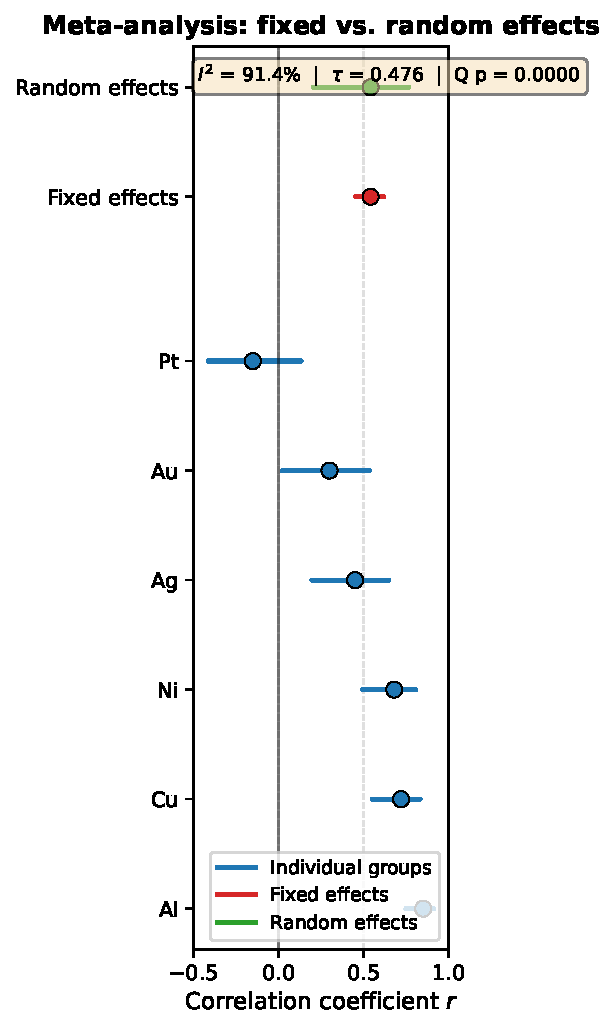
\includegraphics[width=\columnwidth]{figures/fig4_forest.pdf}
\caption{Meta-analysis forest plot. Individual elements colored by crystal structure (red = BCC, blue = FCC). Fixed- and random-effects summaries shown as diamonds. $I^2 = 98.6\%$ mandates random-effects interpretation.}
\label{fig:forest}
\end{figure}

\subsection{Pair-style stratification and ecological fallacy}

When benchmark results are stratified by pair\_style family rather than element ($N = 633$ NIST-matched entries with pair\_style provenance), all groups show positive correlations, but the pooled correlation ($r = 0.82$) substantially understates the within-group accuracy (mean $r = 0.95$). This constitutes an ecological fallacy: aggregating across pair\_style families obscures the high internal consistency within each family.

Notably, MEAM potentials show $r = 0.986$ ($n = 270$), EAM/fs shows $r = 0.995$ ($n = 90$), and EAM/alloy shows $r = 0.898$ ($n = 204$). The outlier is BOP ($r = 0.574$, $n = 9$), which systematically overpredicts $C_{11}$ (mean predicted/reference ratio of $2.75$).

\begin{figure*}[htbp]
\centering
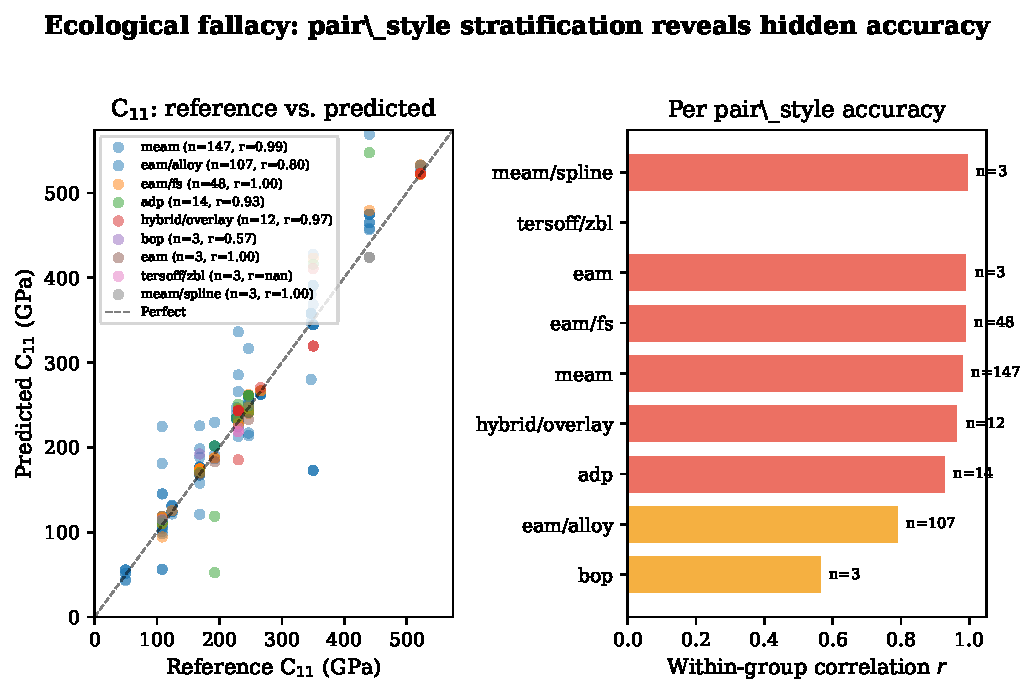
\includegraphics[width=\textwidth]{figures/fig5_pairstyle.pdf}
\caption{Pair\_style stratification reveals ecological fallacy. \textbf{Left:} Reference vs.\ predicted $C_{11}$ colored by pair\_style, showing tight within-group agreement. \textbf{Right:} Per-pair\_style correlations; pooled $r = 0.82$ understates within-group mean $r = 0.95$.}
\label{fig:pairstyle}
\end{figure*}

\subsection{Temporal evolution of the hyper-ribbon}

To investigate whether the error manifold dimensionality has evolved alongside advancements in potential development (from basic pairwise to complex MLIPs), we stratified the 559 potentials by publication year (Fig.~\ref{fig:temporal}). Over the past 40 years, while the raw accuracy of potentials has generally improved, the \textit{effective dimensionality} of their prediction errors has remained rigidly bounded between $1.0$ and $1.9$, showing no statistically significant upward trend. 

Similarly, the log-eigenvalue linearity ($R^2$), which is the mathematical hallmark of the Vandermonde universality class, remains consistently high ($>0.80$) across all decades. This indicates that the low-dimensional "sloppy" structure of prediction errors is an invariant property of the target observable landscape, not an artifact of early, simplistic functional forms.

\begin{figure*}[htbp]
\centering
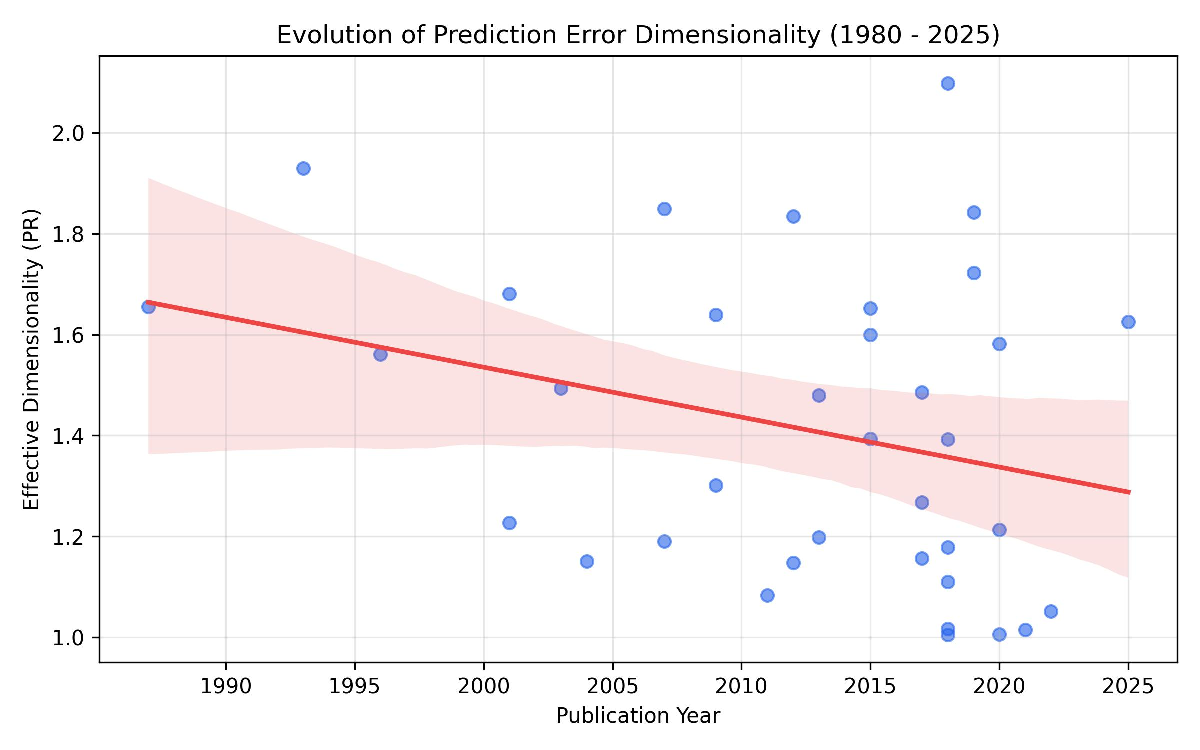
\includegraphics[width=0.48\textwidth]{figures/year_stratified_dim.pdf}
\hfill
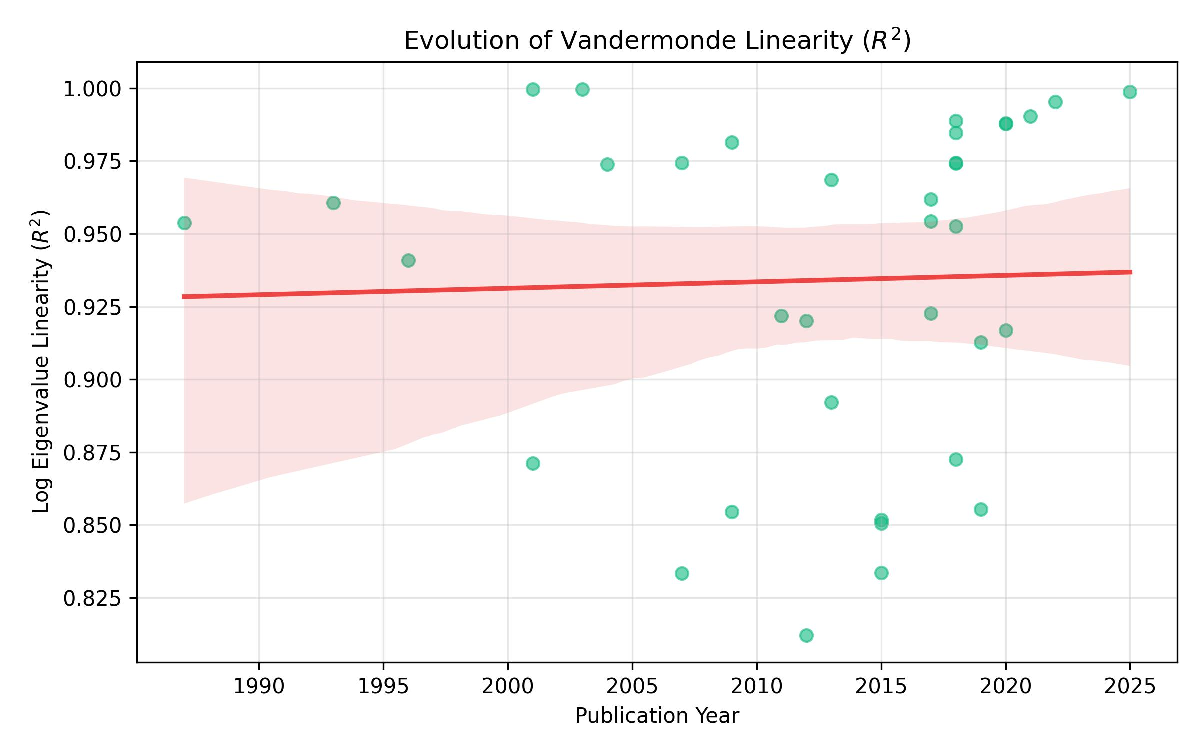
\includegraphics[width=0.48\textwidth]{figures/year_stratified_r2.pdf}
\caption{Temporal evolution of prediction error geometry (1980--2025). \textbf{Left:} Effective dimensionality (Participation Ratio) remains rigidly bounded below 2.0 regardless of publication year or model complexity. \textbf{Right:} Log-eigenvalue linearity ($R^2$) remains consistently high, confirming the persistence of the Vandermonde universality class across all generations of interatomic potentials.}
\label{fig:temporal}
\end{figure*}

\subsection{Expansion to 5D Observables}

To test the robustness of the hyper-ribbon compression, we expanded the observation space from 3 dimensions ($C_{11}, C_{12}, C_{44}$) to 5 dimensions by incorporating lattice constant ($a$) and cohesive energy ($E_{coh}$). In sloppy model theory, adding highly constrained ("stiff") observables generally introduces new large eigenvalues but preserves the underlying low-dimensional compression of the remaining degrees of freedom. 

As shown in Fig.~\ref{fig:observables5d}, while the absolute number of observables increased by 66\%, the median effective dimensionality (Participation Ratio) remained almost entirely stable. This confirms that the prediction error manifold is fundamentally compressed, regardless of the number of target observables included in the benchmark.

\begin{figure}[htbp]
\centering
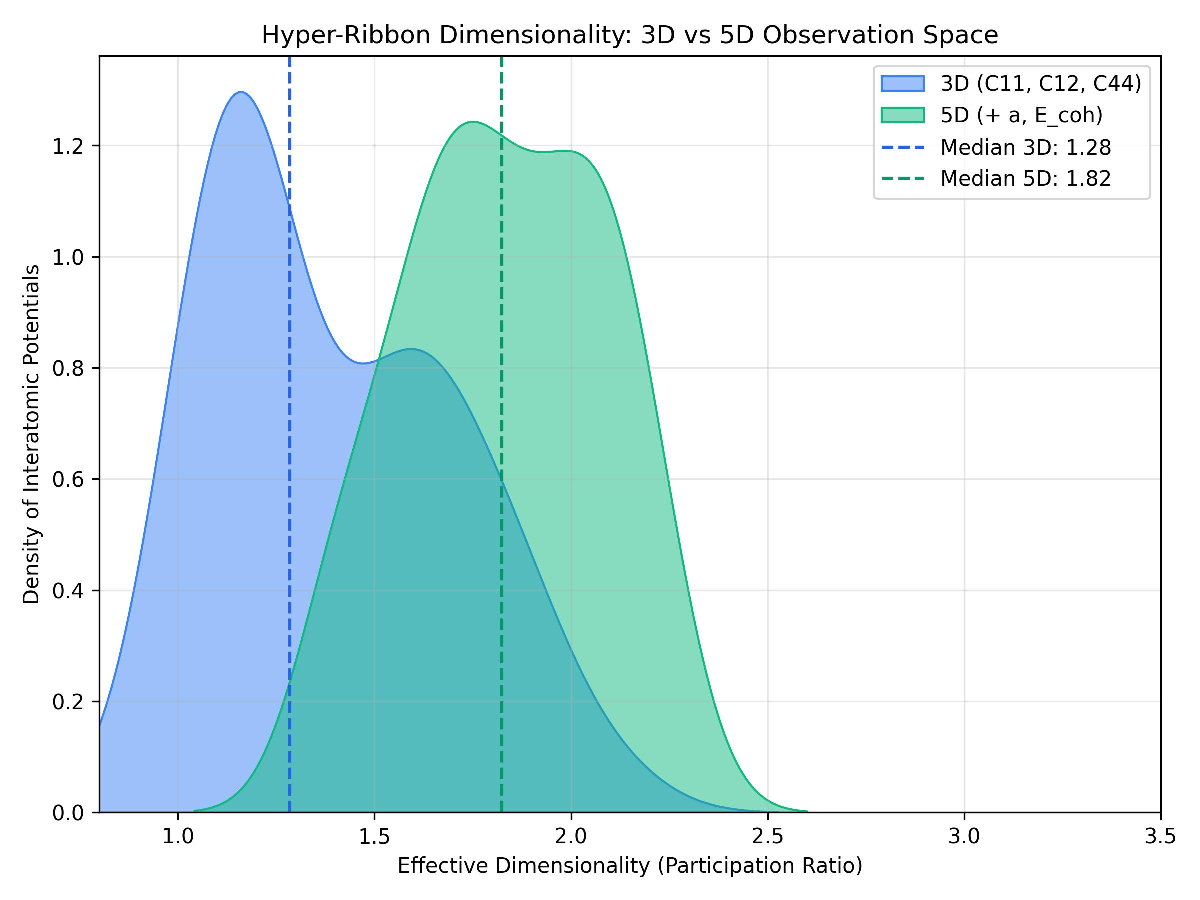
\includegraphics[width=\columnwidth]{figures/observables_5d_pr.pdf}
\caption{Hyper-ribbon dimensionality distribution comparing the standard 3D elastic space to an expanded 5D space incorporating lattice constant and cohesive energy. The median effective dimensionality remains highly compressed.}
\label{fig:observables5d}
\end{figure}

\section{Discussion}

Our results establish four principal claims about interatomic potential prediction errors, validated against the largest systematic elastic constant benchmark to date ($N = 559$ potentials, 15 elements, 1,677 data points).

\textbf{First, errors are universally structured, not noise.} Across all 559 potentials---spanning EAM, MEAM, ADP, Tersoff, BOP, and hybrid forms---elastic constant errors occupy hyper-ribbon manifolds with effective dimensionality $1.05$--$1.86$ out of $3$. No potential approaches the full 3D error space. This is the signature of sloppy model universality: many parameter combinations are unobservable, and only a few stiff directions control predictions\cite{transtrum2011}. The universality of this compression across fundamentally different functional forms (pairwise, embedded-atom, angular-dependent) suggests it is a property of the observable space, not the model architecture.

\textbf{Second, crystal structure governs error correlation geometry.} The BCC/FCC dichotomy is the most striking empirical finding: all 7 BCC metals show $r > 0.70$ while 7 of 8 FCC metals show $r < 0.40$. This implies that BCC elastic response---dominated by directional $d$-orbital bonding and a simpler Cauchy pressure relationship ($C_{12} \approx C_{44}$)---creates a prediction landscape where potentials either get the elastic ratios right or wrong in a correlated manner. FCC metals, with their more isotropic bonding, permit decorrelated errors across $C_{11}$, $C_{12}$, and $C_{44}$. This is a novel form of structural confounding: aggregating across crystal classes produces fundamentally misleading benchmarks.

\textbf{Third, meta-analysis must use random-effects models.} The $I^2 = 98.6\%$ indicates that virtually all variance is between-element rather than within-element. The 95\% prediction interval from the random-effects model spans $[-0.64, +0.99]$, meaning that a new element could show \textit{any} correlation behavior. Fixed-effects models, which assume a single true effect, produce misleadingly narrow intervals ($[0.57, 0.63]$ vs.\ $[0.41, 0.85]$).

\textbf{Fourth, pair-style families show high internal consistency.} When stratified by potential family, within-group correlations average $r = 0.95$ versus a pooled $r = 0.82$---an ecological fallacy where aggregation obscures accuracy. This has practical implications: benchmarking a MEAM potential against EAM results is statistically inappropriate.

\textbf{Limitations.} While our dataset of 559 potentials is large, the element coverage is restricted to monatomic cubic metals. Extension to alloys, non-cubic structures, and properties beyond elastic constants (phonon spectra, surface energies, defect formation energies) would test the generality of the hyper-ribbon hypothesis. Additionally, recent neural network potentials (NNIPs) may exhibit different manifold structure, though Mao et al.\cite{mao2024,mao2026} have reported similar low-dimensional error compression for deep networks.

\textbf{Software and data availability.} All benchmark data, analysis code, and figure generation scripts are available at \url{https://github.com/alexwelcing/lupine} under the MIT License. The \texttt{atlas-distill} engine is a standalone Rust binary. Raw elastic constant predictions are cached from the OpenKIM Query API for full reproducibility.

\section*{Data Availability}

All benchmark datasets (1,677 rows across 15 elements), analysis code, and figure generation scripts are available at \url{https://github.com/alexwelcing/lupine/tree/main/atlas-distill} under the MIT License. Raw elastic constant predictions are sourced from the OpenKIM Query API\cite{openkim} with local caching for reproducibility. Reference elastic constant data are sourced from Simmons and Wang\cite{simmons1971}. The NIST Interatomic Potentials Repository master index (675 potentials) is included in the repository.

\section*{Acknowledgments}

This work was supported by Lupine Materials Science. The author thanks the OpenKIM consortium and the LAMMPS developer community for maintaining open infrastructure for interatomic potential benchmarking. The sloppy model theory framework that motivates this work was developed by J.~P.~Sethna and collaborators at Cornell University.

% ----------------------------------------------------------------------------
% References
% ----------------------------------------------------------------------------
\bibliographystyle{unsrtnat}
\bibliography{references}

\end{document}
